% based on Model 2 of "Activity 10 - Class Design" by Helen Hu

\model{Designing a Class}

Classes are often used to represent abstract data types, such as \java{Color} or \java{String}.
They are also used to represent objects in the real world, such \java{Person} or \java{CreditCard}.
UML class diagrams summarize the attributes and methods of a class.

\begin{center}
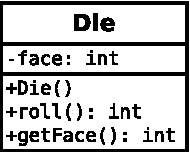
\includegraphics{CS1/Die.pdf}
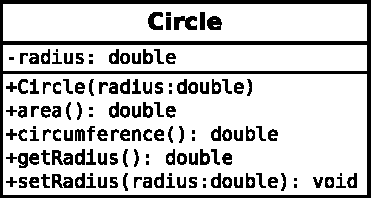
\includegraphics{CS1/Circle.pdf}
\end{center}

Methods in a class generally fall into one of five categories:
\begin{itemize}[itemsep=0pt]
\item \textbf{constructor} methods that initialize new objects
\item \textbf{accessor} methods (getters) that return attributes
\item \textbf{mutator} methods (setters) that modify attributes
\item \textbf{object} methods such as \java{equals} and \java{toString}
\item \textbf{utility} methods which are generally static
\end{itemize}


\quest{15 min}


\Q Identify a mutator method in the Color class.
\begin{enumerate}
\item Which data field did it set?
\item What arguments did the method take?
\item What does the method return?
\end{enumerate}


\Q Identify an accessor method in the Color class. 
\begin{enumerate}
\item Which data field did it get?
\item What arguments did the method take?
\item What does the method return?
\end{enumerate}


\vspace{1em}
For the next few questions, consider a class that will be used to represent an individual's credit card.
\begin{center}
% https://www.bankofamerica.com/credit-cards/
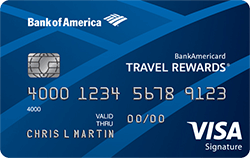
\includegraphics{CS1B/credit-card.png}
\end{center}


\Q Give two data fields that would be appropriate for this CreditCard class.

\begin{enumerate}
\item 
\item 
\end{enumerate}


\Q For each data field, what data type would be appropriate?

\begin{enumerate}
\item 
\item 
\end{enumerate}


\Q Are there any invalid values for the two data fields?

\begin{enumerate}
\item 
\item 
\end{enumerate}


\Q Give two mutator methods would be appropriate for the CreditCard class.
Include arguments and return values, using the same format used for methods in the UML diagram in Model 1.

\begin{enumerate}
\item 
\item 
\end{enumerate}
 

\Q Give two accessor methods would be appropriate for the CreditCard class.
Include arguments and return values, using the same UML format.

\begin{enumerate}
\item 
\item 
\end{enumerate}


\Q Which of your four methods will need to handle invalid values? How would your group like to handle those values? Justify your answer.

\begin{answer}
\end{answer}
